\documentclass[spanish]{mathnotes}

% Title page
\title{Métodos numéricos para EDP}
\subtitle{Métodos upwind y Lax-Wendroff para la ecuación de advección lineal}
\author{Guillermo Ruiz Álvarez}
\date{\today}
\university{Universidad Autónoma de Madrid}

%Theorem name
\mntheoremname{Teorema}
\mnlemmaname{Lema}

\begin{document}
	\makepre
	
	\section{Definición del problema}
	Consideramos el siguiente problema para la ecuación de advección lineal:
	\begin{equation*}
		\left\{
		\begin{array}{l l}
			u_t + a(x,t)u_x = 0 & (x,t) \in (0,1)\times(0,T)\\
			u(0,t) = 0 & t > 0\\
			u(x,0) = u_0(x) & 0\le x\le 1
		\end{array}
		\right.
	\end{equation*}
	donde $a(x,t)$ tiene la siguiente expresión:
	$$a(x,t) = \frac{1+x^2}{1+2xt+2x^2+x^4}$$
	y la condición inicial:
	\begin{equation*}
		u_0(x) = \left\{
		\begin{array}{l l}
		1 & x\in [0.2,0.4]\\
		0 & x\notin [0.2,0.4]
		\end{array}
		\right.
	\end{equation*}
	
	\section{Solución exacta del problema}
	Sea $u(x,t)$ la solución del problema. Para resolverlo utilizamos el método de las características, que vienen dadas por la ecuación:
	$$\frac{\partial x}{\partial t} = a(x,t)$$
	Vemos que la solución es constante a lo largo de las características ya que:
	$$\frac{\partial u(x(t), t)}{\partial t} = 
	u_t + \frac{\partial x}{\partial t}u_x = u_t + a(x,t)u_x = 0$$
	Resolvemos la ecuación de las características:	
	$$x^\prime = \frac{1+x^2}{1+2xt+2x^2+x^4} = \frac{1+x^2}{2xt+(1+x^2)^2}$$
	Agrupando términos
    $$2xx^\prime t+x^\prime(1+x^2)^2 = 1+x^2$$
    y despejando $x^\prime$ obtenemos:
	$$x^\prime = \frac{(1+x^2)-t2xx^\prime}{(1+x^2)^2}$$
	Hallamos así la expresión:
	$$x' = \left(\frac{t}{1+x^2}\right)^\prime$$
	Luego las características satisfacen la ecuación: 
	$$x - \frac{t}{1+x^2} = cte$$
	Dado que la solución es constante a lo largo de las características y tenemos $u(x,0) = u_0(x)$ como condicion inicial, la solución exacta al problema es:
	$$u(x,t) = u(x^*,0) = u_0(x^*) = u_0\left(x - \frac{t}{1+x^2}\right)$$
	\subsection{Programación de la solución}
	Para programar la solución exacta del problema se ha escrito el siguiente código en \textsc{Matlab} utilizando lo visto en el apartado anterior:
	\lstset{style=matlabStyle}
	\lstinputlisting{../src/adveq_sol.m}
	
	\section{Solución utilizando métodos numéricos}
	En esta sección se va a realizar una aproximación a la solución del problema de advección lineal mediante dos métodos numéricos: el esquema upwind y el método Lax-Wendroff. En todo lo que sigue se considerará un mallado equiespaciado tanto para la variable espacial como para la temporal, además, se tomará
	$$\Delta x = \Delta t$$
	
	Para cada método se realizarán 6 aproximaciones con los datos siguientes:  espaciado del mallado $\Delta x=\Delta t = 0.02$ y $\Delta x=\Delta t = 0.01$ en tiempos $T =$ 0.1, 0.5 y 1.
	
	\subsection{Método upwind}
	En este apartado se estudiará el método upwind y los resultados que ofrece para la resolución del problema de advección lineal.
	
	Dado que $a>0$, el método tiene la expresión siguiente: 
	$$\frac{U_{j}^{n+1}-U_{j}^{n}}{\Delta t} + a_j^n\frac{U_{j}^{n}-U_{j-1}^{n}}{\Delta x} = 0$$
	Que teniendo en cuenta que $\Delta x = \Delta t$, tiene la siguiente forma explícita:
	$$U_{j}^{n+1} = U_j^n - a_j^n \left(U_j^n - U_{j-1}^n\right)$$
	
	Se estudiará la condición Courant-Friedrich-Levy (CFL), la consistencia y estabilidad del esquema, se comprobará si cumple el principio del máximo y finalmente se presentarán los resultados obtenidos.
	
	\subsubsection{Condición CFL}
	Vamos a comprobar si se satisface la condición CFL, que dice que el dominio de dependencia teórico ha de estar contenido en el dominio de dependencia numérico.
		\begin{figure}[ht]
			\centering
			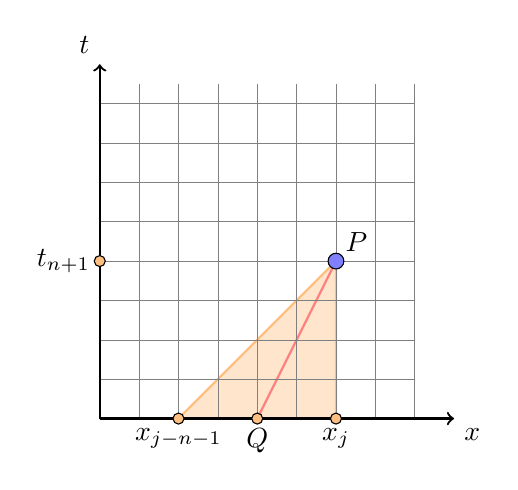
\begin{tikzpicture}[domain=0:4]
			%Triangle
			\draw[thick, -, orange!50!white] (1, 0) -- (3,2);
			\draw [thick,-,orange!50!white, fill=orange!20!white] (1,0)--(3,2)--(3,0)--cycle;
			\draw[thick, -, red!50!white] (2, 0) -- (3,2);
			%Grid
			\draw[step=5mm,very thin,color=gray] (0,0) grid (4,4.25);
			%Axis
			\draw[thick,->] (0,0) -- (4.5,0) node[below right] {$x$};
			\draw[thick,->] (0,0) -- (0,4.5) node[above left] {$t$};
			\draw[fill=blue!50!white, draw=black] (3,2) circle (1mm) node[above right]{$P$};
			\draw[fill=orange!50!white, draw=black] (3,0) circle (0.7mm) node[below]{$x_{j}$};
			\draw[fill=orange!50!white, draw=black] (1,0) circle (0.7mm) node[below]{$x_{j-n-1}$};
			\draw[fill=orange!50!white, draw=black] (0,2) circle (0.7mm) node[left]{$t_{n+1}$};
			\draw[fill=orange!50!white, draw=black] (2,0) circle (0.7mm) node[below]{$Q$};
			\end{tikzpicture}
			\caption{Condición CFL}
			\label{fig:cfl_1}
		\end{figure}
		
	\noindent Dado el esquema upwind:
	$$\frac{U_{j}^{n+1}-U_{j}^{n}}{\Delta t} + a_j^n\frac{U_{j}^{n}-U_{j-1}^{n}}{\Delta x} = 0$$
	Tomando $\nu = \frac{a \Delta t}{\Delta x}$ obtenemos la expresión:
	$$U_j^{n+1} = (1-\nu)U_j^n + \nu U_{j-1}^n$$
	El valor de $U_j^{n+1}$ depende de la condición inicial en los puntos $\left\{x_{j-n-1}, \hdots, x_j\right\}$ cuando $t=0$ (ver figura \ref{fig:cfl_1}).
	Para que el dominio de dependencia teórico quede contenido en el dominio de dependencia numérico es necesario que el punto $Q=(x_j-at_{n+1}, 0)$ quede en el intervalo $[x_{j-n-1}, x_j]$. El segmento $\overline{PQ}$, que tiene pendiente $\frac{1}{a}$, tiene que quedar dentro del triángulo, esto es, se tiene que cumplir que:
	$$\frac{\Delta t}{\Delta x} \le \frac{1}{a}$$
	Dado que $\Delta x = \Delta t$, esto es lo mismo que decir que:
	$$a \le 1$$
	Lo cual siempre ocurre en el dominio puesto que para $x>0$ y $t>0$:
	$$a = \frac{1+x^2}{1+2xt+2x^2+x^4} =  \frac{1+x^2}{(1+x^2)+2xt+x^2+x^4} \le 1$$
	\subsubsection{Consistencia del método}
	El error de truncación tiene la forma:
	$$T_j^n = \frac{u_{j}^{n+1}-u_{j}^{n}}{\Delta t} + a_j^n\frac{u_{j}^{n}-u_{j-1}^{n}}{\Delta x}$$
	Realizamos los desarrollos de Taylor de ambos términos:
	\begin{align*}
	\frac{u_{j}^{n+1}-u_{j}^{n}}{\Delta t} &= (u_t + \frac{1}{2}u_{tt}\Delta t+\hdots)_j^n\\
	\frac{u_{j}^{n}-u_{j-1}^{n}}{\Delta x} &= (u_x - \frac{1}{2}u_{xx}\Delta x+\hdots)_j^n
	\end{align*}
	Nos queda la siguiente expresión para el error de truncación:
	$$T_j^n = \left(u_t+\frac{1}{2} u_{tt}\Delta t+ a \left[u_{x}-\frac{1}{2} u_{xx}\Delta x\right]+\hdots\right)_j^n$$
	Aplicando la ecuación de advección lineal obtenemos:
	$$T_j^n = \left( \underbrace{u_t+au_x}_{0}+\frac{1}{2} u_{tt}\Delta t-\frac{1}{2} a u_{xx}\Delta x+\hdots\right)_j^n$$
	Tenemos por tanto que el método es consistente de primer orden tanto en la variable temporal como en la variable espacial.	
	\subsubsection{Estabilidad del método}
	Se va a estudiar la estabilidad del método realizando un análisis de Fourier para ver cual es el factor de amplificación $\lambda$.
	En primer lugar, tenemos que la condición inicial tiene la expresión:
	$$u_0(x) = \sum_{m=-\infty}^{\infty}b_m e^{im\pi x}$$
	Y dado que la solución general es un desplazamiento del valor inicial se tiene
	$$u(x_j, t_n) = u_0(x_j-a t_n)= \sum_{m=-\infty}^\infty b_me^{im\pi (x_j-a t_n)}$$
	Luego nos queda la expresión: 
	$$u(x_j, t_n) = \sum_{m=-\infty}^\infty b_m\left[e^{-im\pi a \Delta t}\right]^ne^{im\pi j \Delta x}$$
	Dado que $a>0$, si tomamos $\nu = \frac{a\Delta t}{\Delta x}$ el método tiene la forma:
	$$U_{j}^{n+1} = (1-\nu)U_{j}^{n}+\nu U_{j-1}^{n}$$
	Así que, tomando $k=m\pi$, buscamos el factor de amplificación $\lambda$ de manera que:
	$$U_{j}^{n}=\lambda ^n e^{ikj\Delta x}$$ 
	Ahora sustituimos en la expresión del esquema y obtenemos:
	$$\lambda^{n+1}e^{ikj\Delta x} = (1-\nu) \lambda ^n e^{ikj\Delta x}+\nu \lambda^ne^{ik(j-1)\Delta x}$$
	Dividimos por $\lambda^ne^{ikj\Delta x}$ y despejamos $\lambda$:
	$$\lambda = (1-\nu) + \nu e^{-ik\Delta x} = \left[(1-\nu)+\nu \cos(k\Delta x)\right] + i\nu \sin(k\Delta x)$$
	Como siempre, tenemos estabilidad si y solo si $|\lambda|\le 1$, puesto que si no la serie divergería. Para que los cálculos sean más sencillos, vamos a hallar el valor del cuadrado del módulo $\lambda$:
	\begin{align*}
		|\lambda|^2 &= \left[(1-\nu)+\nu \cos(k\Delta x)\right]^2 +\nu^2\sin^2(k\Delta x)\\
		&= (1-\nu)^2+\nu^2\cos^2(k\Delta x) + 2\nu(1-\nu)\cos(k\Delta x)+\nu^2 \sin^2(k\Delta x)\\
		&= (1-\nu)^2 + \nu^2 + 2\nu(1-\nu)\cos(k\Delta x)\\
		&= 1-2\nu(1-\nu)(1-\cos(k\Delta x))\\
		&= 1-4\nu (1-\nu)\sin^2\left(\frac{k\Delta x}{2}\right) \le 1-4\nu (1-\nu)\\
	\end{align*}
	Luego la condición de estabilidad es $1-4\nu (1-\nu)\le 1$ que es equivalente a que
	$$\nu \le 1$$
	Obtenemos que la condición de estabilidad coincide con la condición CFL, por tanto, el método es estable.
	\subsubsection{Principio del máximo}
	Dado el esquema upwind 
	$$U_{j}^{n+1} = (1-\nu)U_{j}^{n}+\nu U_{j-1}^{n}$$
	y asumiendo la condición CFL
	$$\nu \le 1$$
	podemos observar que los términos $(1-\nu)$ y $\nu$ son no negativos y suman $1$. Tenemos entonces que el valor de $U_j^{n+1}$ viene dado como una combinación convexa de los valores $U_j^n$ y $U_{j-1}^n$ y por tanto estará entre los valores máximo y mínimo de estos dos reales. Con esto se llega a que el esquema cumple el principio del máximo. 
	\subsubsection{Programación del método}
	A continuación se muestra el código escrito en \textsc{Matlab} del esquema upwind.
	\lstset{style=matlabStyle}
	\lstinputlisting{../src/upwind.m}
	En el código del método se utiliza una función para calcular el valor de $a$ en cada paso del mismo. El código de la función $a$ es el siguiente:
	\lstset{style=matlabStyle}
	\lstinputlisting{../src/a.m}
	\subsubsection{Resultados obtenidos}
	Una vez programado el método, se han ejecutado las pruebas para obtener las aproximaciones de la solución del problema de advección lineal para los datos dados. 
	\begin{center}
	\begin{figure}
		\makebox[\textwidth][c]{
			\begin{subfigure}{.7\textwidth}
				\centering
				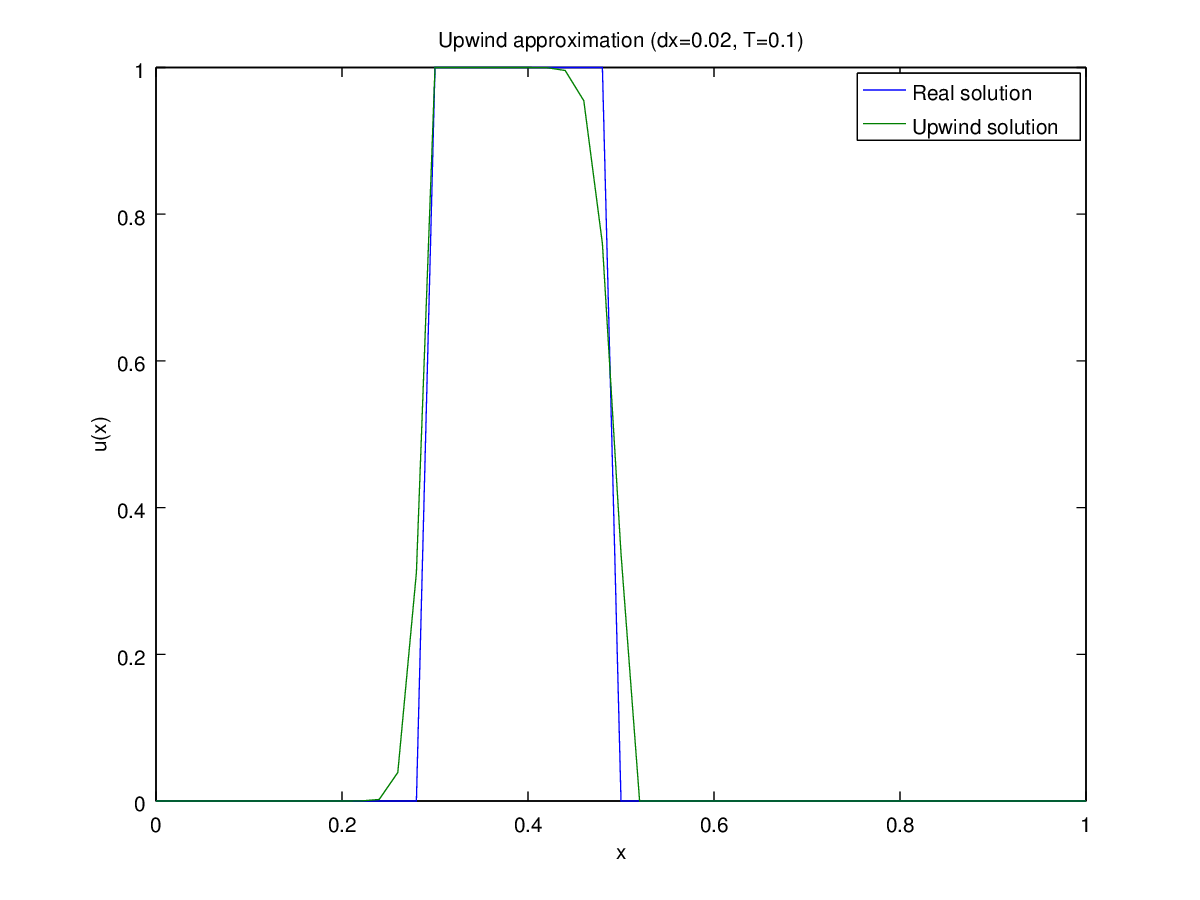
\includegraphics[width=1\linewidth]{../img/upwind_1.png}
				\caption{$\Delta x = 0.02$, $T = 0.1$}
				\label{fig:sfig1}
			\end{subfigure}%
			\begin{subfigure}{.7\textwidth}
				\centering
				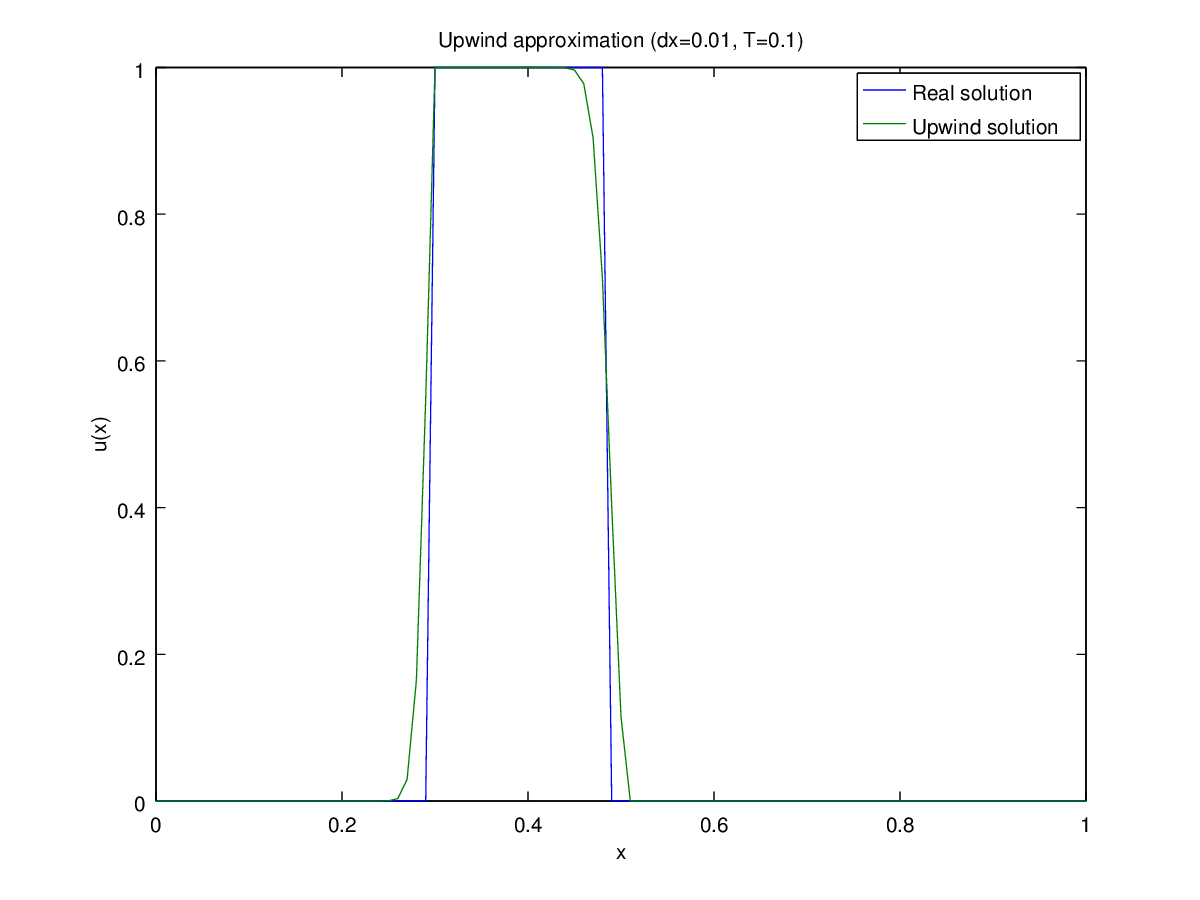
\includegraphics[width=1\linewidth]{../img/upwind_4.png}
				\caption{$\Delta x = 0.01$, $T = 0.1$}
				\label{fig:sfig4}
			\end{subfigure}%
		}
				
		\makebox[\textwidth][c]{
			\begin{subfigure}{.7\textwidth}
				\centering
				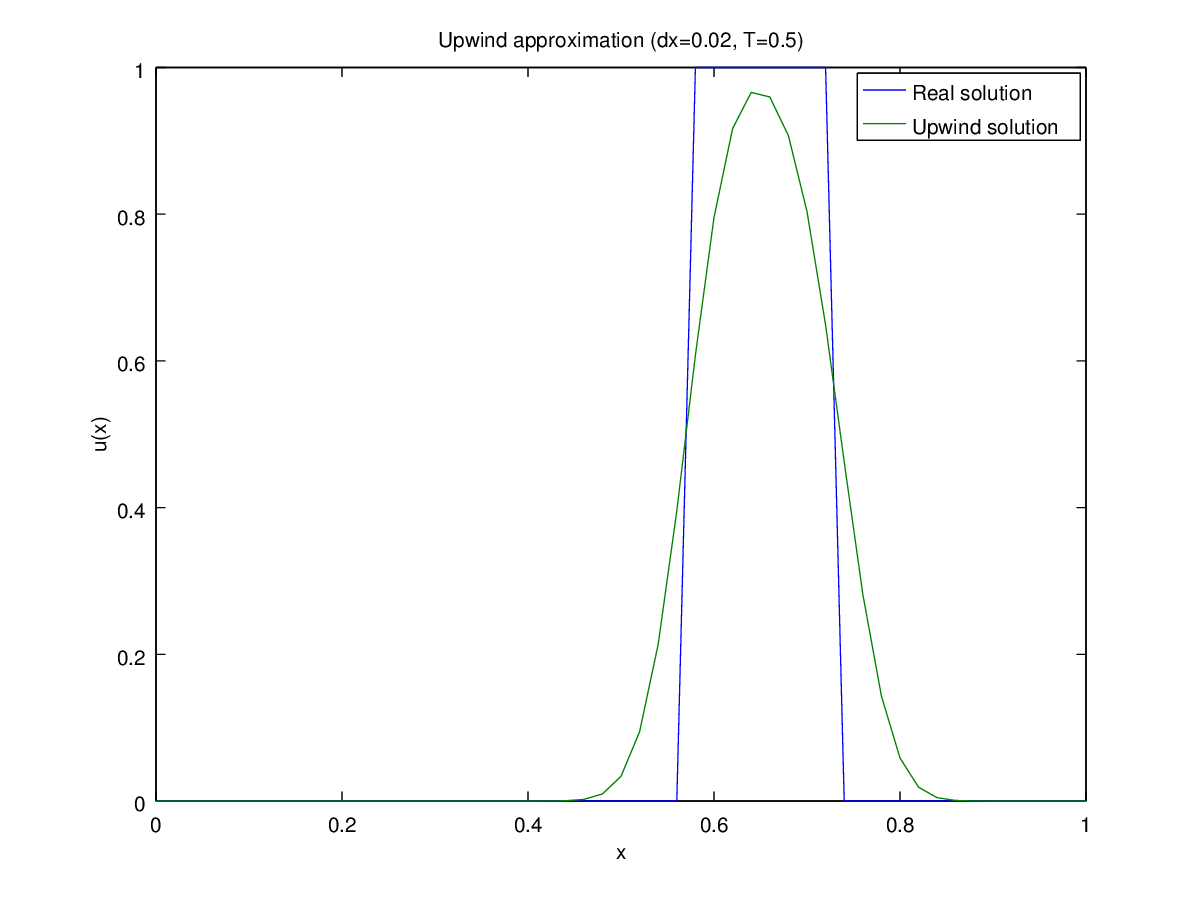
\includegraphics[width=\linewidth]{../img/upwind_2.png}
				\caption{$\Delta x = 0.02$, $T = 0.5$}
				\label{fig:sfig2}
			\end{subfigure}%
			\begin{subfigure}{.7\textwidth}
				\centering
				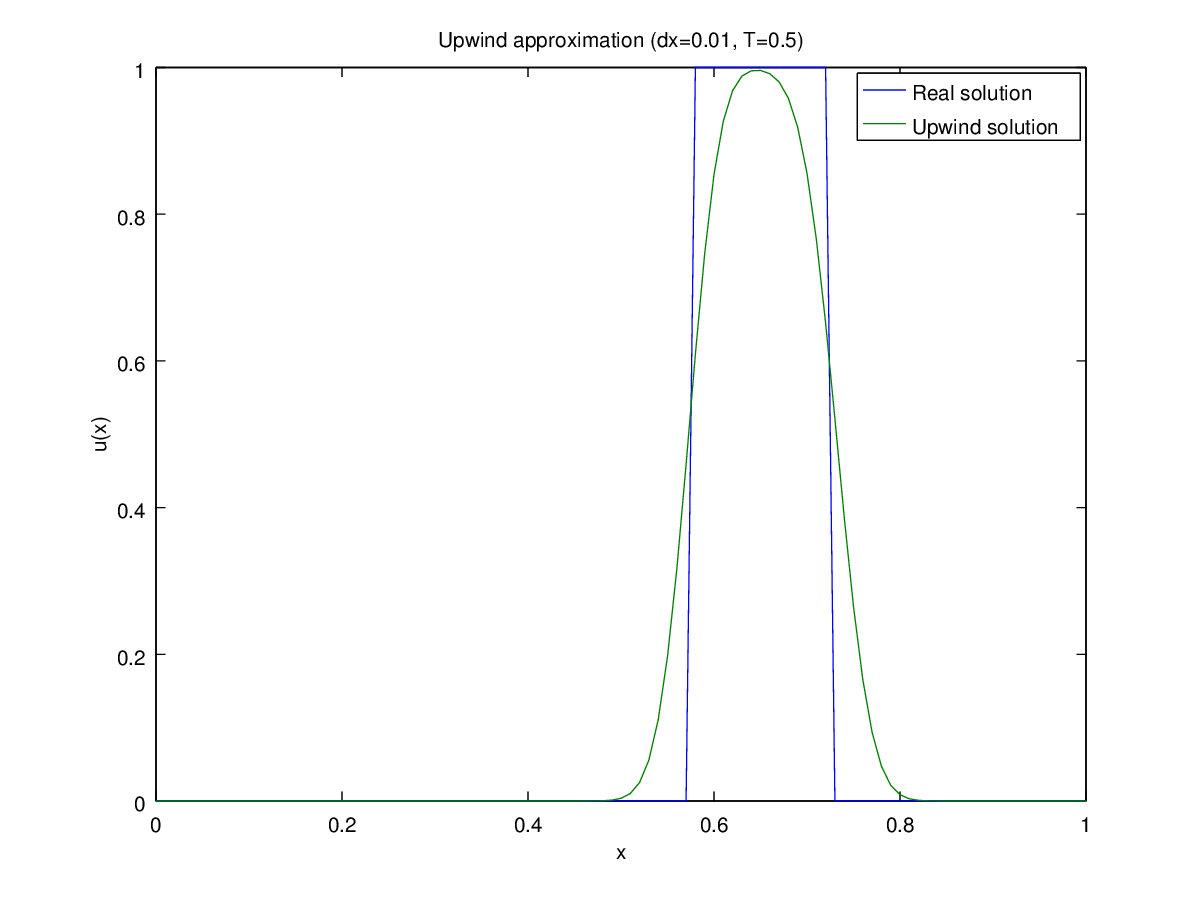
\includegraphics[width=1\linewidth]{../img/upwind_5.png}
				\caption{$\Delta x = 0.01$, $T = 0.5$}
				\label{fig:sfig5}
			\end{subfigure}%
		}
		
		\makebox[\textwidth][c]{
			\begin{subfigure}{.7\textwidth}
				\centering
				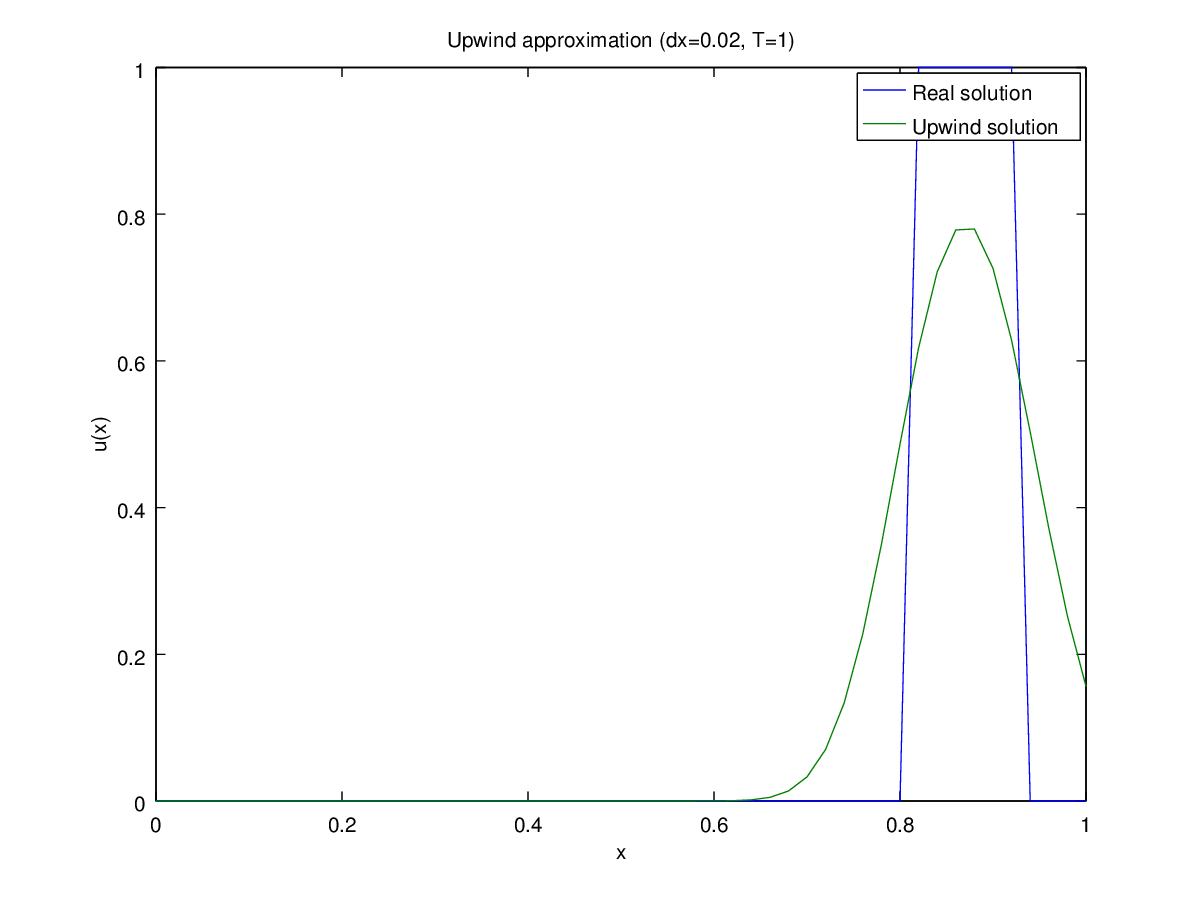
\includegraphics[width=1\linewidth]{../img/upwind_3.png}
				\caption{$\Delta x = 0.02$, $T = 1$}
				\label{fig:sfig3}
			\end{subfigure}%
			\begin{subfigure}{.7\textwidth}
				\centering
				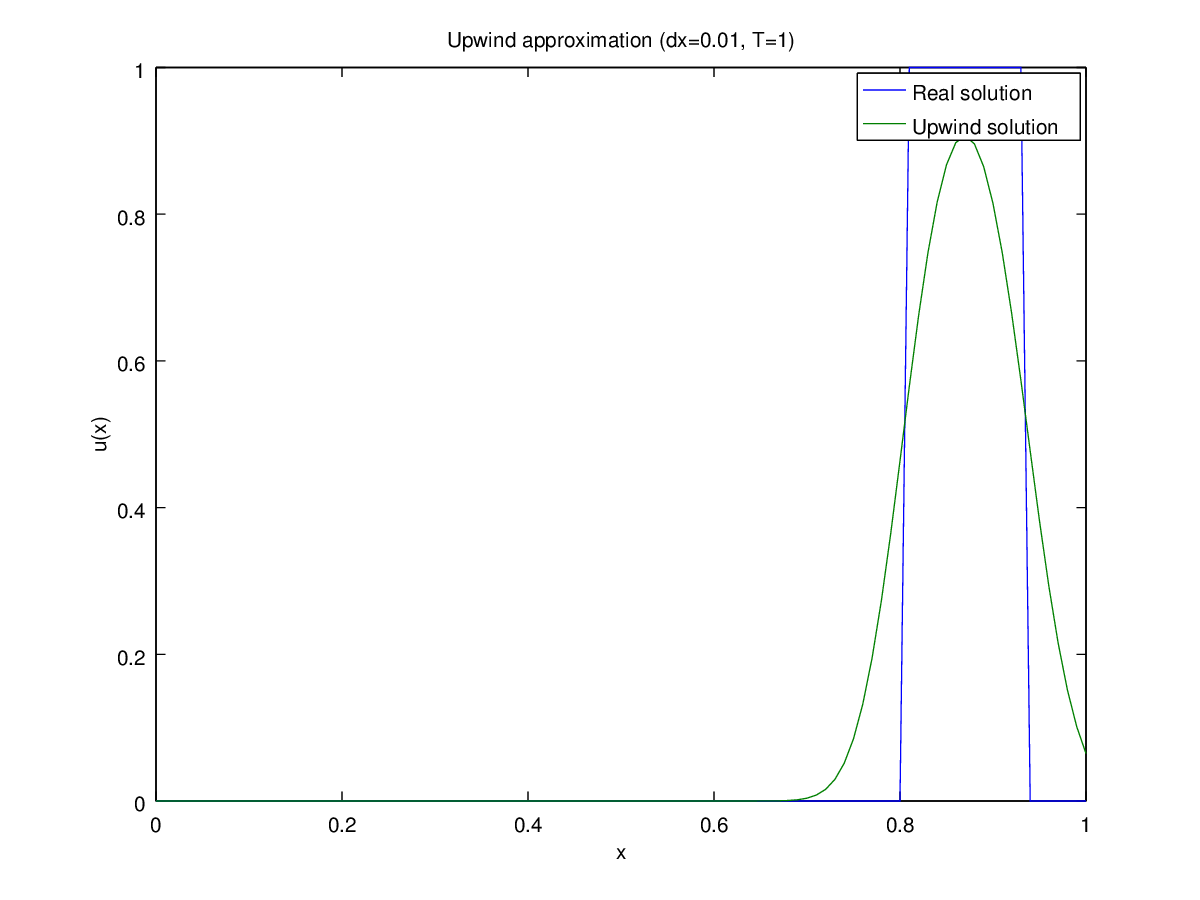
\includegraphics[width=1\linewidth]{../img/upwind_6.png}
				\caption{$\Delta x = 0.01$, $T = 1$}
				\label{fig:sfig6}
			\end{subfigure}%
		}
		\caption{Advección lineal utilizando el método upwind.}
		\label{fig:sfig_upwind}
	\end{figure}
	\end{center}
	
	Sabemos que el modo teórico del esquema es $e^{-ik at}$ y que el factor de amplificación tiene la expresión $\lambda(k) = 1-(1-\nu) e^{-ik\Delta x}$. Analizamos el módulo del factor de amplificación:
	$$|\lambda(k)|^2= 1-4\nu (1-\nu)\sin^2\left(\frac{k\Delta x}{2}\right)$$
	Para frecuencias bajas, se tiene que el error en módulo es $\mathcal{O}((k\Delta x)^2)$. Para la frecuencia mas alta, se tiene que $|\lambda(k)| = \sqrt{1-4\nu(1-\nu)}$. 
	A medida que $n$ aumenta, la solución numérica tiene menos modos de altas frecuencias.
	En cuanto al error en fase, sabemos que la fase teórica es $-ka\Delta t$. 
	Dado que 
	$$\lambda(k)=\left[(1-\nu)+\nu \cos(k\Delta x)\right] + i\nu \sin(k\Delta x)$$
	La fase numérica tiene la expresión:
	$$\arctan(\lambda(k)) = -\arctan\left(\frac{\nu \sin(k\Delta x)}{(1-\nu)+\nu \cos(k\Delta x)}\right)$$
	Vamos a utilizar el desarrollo de la serie de Taylor y el lema que sigue:
	\begin{lemma}
		Si $q=c_1p+c_2p^2+c_3p^3+\hdots$, entonces
		$$\arctan(q) = c_1p+c_2p^2+(c_3-\frac{1}{3}c_1^3)p^3+\hdots$$
	\end{lemma}
	Para obtener:
	$$\arctan(\lambda(k)) = -ak\Delta t\left[1-\frac{1}{6}(1-\nu)(1-2\nu)(k\Delta x)^2+\hdots \right]$$
	Para cualquier $k$, si $\nu \neq 1$ y $\nu \neq \frac{1}{2}$, el error relativo en la fase es $\mathcal{O}((h\Delta x)^2)$.
	En la figura \ref{fig:sfig_upwind} se puede observar que los modos de frecuencias altas causan que se regularice la solución numérica y caiga la altura de la misma. Al disminuir el paso espacial a la mitad, se observan mejores resultados pero aun así sigue ocurriendo lo mismo. Por otro lado, debido al pequeño error cometido en fase, se puede observar que la solución numérica se mueve con la velocidad correcta.
	
	
	
	
	
	
	
	
	
	\subsection{Método Lax-Wendroff}
	En este apartado se estudiará el método Lax-Wendroff y los resultados que ofrece para la resolución del problema de advección lineal. Como hasta ahora, tomemos $\nu = \frac{a\Delta t}{\Delta x}$, el método tiene la siguiente expresión:
	$$U_j^{n+1} = U_j^n - \frac{\nu}{2}\left[U_{j+1}^n-U_{j-1}^n\right] + \frac{\nu^2}{2}\left[U_{j+1}^{n}-2U_{j}^{n}+U_{j-1}^{n}\right]$$
	Se estudiará la condición CFL, la consistencia y estabilidad del método, se comprobará si cumple el principio del máximo y finalmente se presentarán los resultados obtenidos.
	Partimos de la serie de Taylor:
	$$u(x,t+\Delta t) = \left.\left(u+u_t\Delta t + \frac{u_{tt}}{2}(\Delta t )^2 + \mathcal{O}((\Delta t)^3)\right)\right|_{(x,t)}$$
	Ahora utilizamos la ecuación del problema de advección que dice que $u_t = -au_x$ para obtener
	\begin{align*}
		u_{tt} &= -(au_x)_t = -(a_tu_x+au_{xt})\\
		&= -a_tu_x-au_{xt} = -a_tu_x-a(u_t)_x\\
		&= -a_tu_x-a(-au_x)_x = -a_tu_x+a(au_x)_x
	\end{align*}
	Sustituimos en el desarrollo de Taylor y obtenemos:
	$$U_{j}^{n+1}-U_{j}^{n} = -a_j^n\Delta t\frac{\Delta_{0x}U_{j}^{n}}{\Delta x}+\frac{1}{2}(\Delta t)^2\left[-(a_t)_j^n\frac{\Delta_{0x}U_{j}^{n}}{\Delta x}+\frac{a_j^n\delta_x(a_j^n\delta_xU_{j}^{n})}{(\Delta x)^2}\right]$$
	donde
	\begin{align*}
		\Delta_{0x} v(x) &= \frac{1}{2}\left[v\left(x+\Delta x\right)-v\left(x-\Delta x\right)\right]\\
		\delta_x v(x) &= v\left(x+\frac{\Delta x}{2}\right)-v\left(x-\frac{\Delta x}{2}\right)
	\end{align*}
	Vamos a desarrollar el método. Partimos de que:
	\begin{align*}
		\Delta_{0x}U_j^n &= \frac{1}{2}\left[U_{j+1}^{n}-U_{j-1}^{n}\right]\\
		a_j^n\delta_xU_j^n &= a_j^n\left[U_{j+\frac{1}{2}}^{n}-U_{j-\frac{1}{2}}^{n}\right]
	\end{align*}
	Calculamos:
	$$\delta_x\left[a_j^n \delta_xU_{j}^{n}\right] = a_{j+\frac{1}{2}}^n \left[U_{j+1}^{n}-U_{j}^{n}\right] -  a_{j-\frac{1}{2}}^n \left[U_{j}^{n}-U_{j-1}^{n}\right]$$
	Y tenemos la expresión:
	\begin{align*}
		U_{j}^{n+1} &= U_{j}^{n} -\frac{a_j^n\Delta t}{\Delta x}\left[\frac{U_{j+1}^{n}-U_{j-1}^{n}}{2}\right]\\
		&+ \frac{(\Delta t)^2}{2}\left(-(a_t)_j^n\left[\frac{U_{j+1}^n-U_{j-1}^n}{2\Delta x}\right]\right)\\
		&+ \frac{(\Delta t)^2}{2}\left(a_j^n\left[a_{j+\frac{1}{2}}^n\left[\frac{U_{j+1}^n-U_j^n}{(\Delta x)^2}\right]-a_{j-\frac{1}{2}}^n\left[\frac{U_{j}^{n}-U_{j-1}^{n}}{(\Delta x)^2}\right]\right]\right)
	\end{align*}
	Aplicando el hecho de que $\Delta x = \Delta t$ y la simplificación que sigue:
	$$a_j^n + \frac{1}{2}({a_t})_j^n \Delta t \approx a_j^{n+\frac{1}{2}}$$
	Se obtiene:
	$$U_j^{n+1} = U_j^n - \frac{a_j^{n+\frac{1}{2}}}{2}\left[U_{j+1}^{n}-U_{j-1}^{n}\right]+\frac{a_j^n}{2}\left[a_{j+\frac{1}{2}}(U_{j+1}^{n}-U_{j}^{n})-a_{j-\frac{1}{2}}^n (U_j^n-U_{j-1}^{n})\right]$$
	Reagrupando términos:
	\begin{align*}
		U_j^{n+1} &= \left[\frac{a_j^{n+\frac{1}{2}}}{2}+\frac{1}{2}a_j^na_{j-\frac{1}{2}}^n\right]U_{j-1}^{n}\\
		&+ \left[1+\frac{1}{2}a_j^n(-a_{j+\frac{1}{2}}^n-a_{j-\frac{1}{2}}^n)\right]U_j^n\\
		&+ \left[-\frac{a_j^{n+\frac{1}{2}}}{2}+\frac{1}{2}a_j^na_{j+\frac{1}{2}}^n\right]U_{j+1}^n
	\end{align*}
	Expresión que implementaremos para el método.
	\subsubsection{Condición CFL}
		Vamos a comprobar si se satisface la condición CFL, que dice que el dominio de dependencia teórico ha de estar contenido en el dominio de dependencia numérico.
		\begin{figure}[ht]
			\centering
			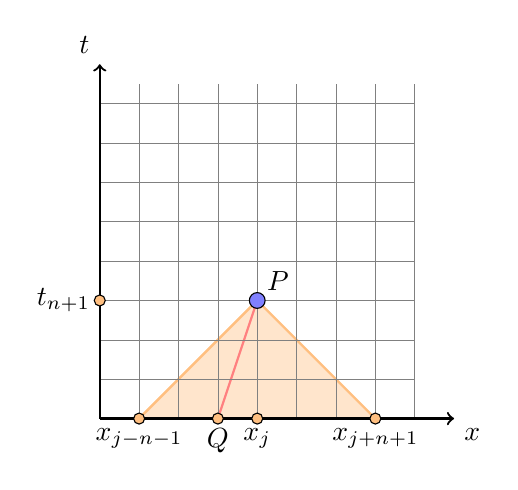
\begin{tikzpicture}[domain=0:4]
			%Triangle
			\draw[thick, -, orange!50!white] (0.5, 0) -- (2,1.5);
			\draw [thick,-,orange!50!white, fill=orange!20!white] (0.5,0)--(2,1.5)--(3.5,0)--cycle;
			\draw[thick, -, red!50!white] (1.5, 0) -- (2,1.5);
			%Grid
			\draw[step=5mm,very thin,color=gray] (0,0) grid (4,4.25);
			%Axis
			\draw[thick,->] (0,0) -- (4.5,0) node[below right] {$x$};
			\draw[thick,->] (0,0) -- (0,4.5) node[above left] {$t$};
			\draw[fill=blue!50!white, draw=black] (2,1.5) circle (1mm) node[above right]{$P$};
			\draw[fill=orange!50!white, draw=black] (3.5,0) circle (0.7mm) node[below]{$x_{j+n+1}$};
			\draw[fill=orange!50!white, draw=black] (0.5,0) circle (0.7mm) node[below]{$x_{j-n-1}$};
			\draw[fill=orange!50!white, draw=black] (0,1.5) circle (0.7mm) node[left]{$t_{n+1}$};
			\draw[fill=orange!50!white, draw=black] (1.5,0) circle (0.7mm) node[below]{$Q$};
			\draw[fill=orange!50!white, draw=black] (2,0) circle (0.7mm) node[below]{$x_j$};
			\end{tikzpicture}
			\caption{Condición CFL}
			\label{fig:cfl_2}
		\end{figure}
		En este caso, el valor de $U_j^{n+1}$ depende de la condición inicial en los puntos $\left\{x_{j-n-1}, \hdots, x_{j+n+1}\right\}$ cuando $t=0$ (ver figura \ref{fig:cfl_2}).
		Para que el dominio de dependencia teórico quede contenido en el dominio de dependencia numérico es necesario que el punto $Q=(x_j-at_{n+1}, 0)$ quede dentro de dicho intervalo. Como tenemos que $a>0$ siempre, el segmento $\overline{PQ}$ tendrá siempre pendiente positiva $\frac{1}{a}$. Se tiene que cumplir que:
		$$\frac{\Delta t}{\Delta x} \le \frac{1}{a}$$
		Dado que $\Delta x = \Delta t$, esto es lo mismo que decir que:
		$$a \le 1$$
		Lo cual ya hemos visto que se cumple en el dominio del problema.
	\subsubsection{Consistencia del método}
	Tal y como se ha construido el método, dada la aproximación de las derivadas por diferencias finitas, se tiene que el método tiene orden 2 de consistencia tanto en la variable espacial como en la variable temporal. El error de truncación tiene la siguiente expresión:
	$$T_j^n = (u_j^{n+1}-u_j^n) + \frac{\nu}{2}(u_{j+1}^n-u_{j+1}^n) - \frac{\nu^2}{2}(u_{j+1}^n-2u_j^n+u_{j-1}^n)$$
	Realizamos los desarrollos de Taylor de los términos:
	\begin{align*}
		u_j^{n+1} & = \left(u+u_t\Delta t + \frac{1}{2}u_{tt}(\Delta t)^2 + \mathcal{O}((\Delta t)^3)\right)_j^n\\
		u_{j+1}^n & = \left(u+u_x\Delta x + \frac{1}{2}u_{xx}(\Delta x)^2 + \mathcal{O}((\Delta x)^3)\right)_j^n\\
		u_{j-1}^n & = \left(u-u_x\Delta x + \frac{1}{2}u_{xx}(\Delta x)^2 + \mathcal{O}((\Delta x)^3)\right)_j^n
	\end{align*}
	Por tanto
	\begin{align*}
	T_j^n &= u_t\Delta t + \frac{1}{2}u_{tt}(\Delta t)^2 + \mathcal{O}((\Delta t)^3)\\
	&+\frac{a\Delta t}{2\Delta x}\left[2u_x\Delta x + \mathcal{O}((\Delta x)^3)\right]\\
	&-\frac{(a\Delta t)^2}{2(\Delta x)^2}\left[u_{xx}(\Delta x)^2+\mathcal{O}((\Delta x)^3)\right]
	\end{align*}
	Reagrupando términos y utilizando la ecuación de advección que dice que $u_t + au_x = 0$ y el hecho de que $\Delta x = \Delta t$ obtenemos:
	$$T_j^n = \left((\underbrace{u_t+au_x}_{=0})\Delta t + \frac{1}{2}u_{tt}(\Delta t)^2 -a^2u_{xx}(\Delta t)^2 + \hdots\right)_j^n$$
	Luego el error del método es $\mathcal{O}((\Delta x)^2 +(\Delta t)^2)$.
	
	\subsubsection{Estabilidad del método}
	Igual que en el caso anterior, buscamos $\lambda(k)$ tal que $$U_j^n = \lambda ^n e^{ikj\Delta x}$$
	Sustituyendo en el método y dividiendo por $\lambda^n e^{ikj\Delta x}$ obtenemos:
	$$\lambda(k) = 1 - \frac{\nu}{2}\left[e^{ik\Delta x}-e^{-ik\Delta x}\right]+\frac{\nu^2}{2}\left[e^{ik\Delta x}-2+e^{-ik\Delta x}\right]$$
	Tomando complejos:	
	$$\lambda(k) = \left(1-2\nu^2sin^2\left(\frac{k}{2}\Delta x\right)\right)-i\nu sin(k\Delta x)$$
	Estudiamos el cuadrado del módulo del factor de amplificación:
	$$|\lambda|^2 = 1-4\nu^2(1-\nu^2)sin^4\left(\frac{k}{2}\Delta x\right)$$
	Tenemos estabilidad si 
	$$|\lambda|\le 1 \iff |\nu| \le 1$$
	que coincide con la condición CFL.
	\subsubsection{Principio del máximo}
	\begin{thm}[Teorema de Godunov]
		Si un esquema lineal para la ecuación $$u_t+au_x = 0$$
		cumple el principio del máximo, entonces no puede tener orden mayor que uno.
	\end{thm}
	Partiendo del teorema de Godunov y dado que el orden del método es cuadrático, podemos concluir que el esquema Lax-Wendroff no puede cumplir el principio del máximo.\newpage
	\subsubsection{Programación del método}
	A continuación se muestra el código escrito en \textsc{Matlab} del esquema Lax-Wendroff.
	\lstset{style=matlabStyle}
	\lstinputlisting{../src/lw.m}
	El código de la función para calcular el valor de $a$ es el mismo que se ha utilizado en el método anterior.
	\subsubsection{Resultados obtenidos}
	Una vez programado el método, se han ejecutado las pruebas para obtener las aproximaciones de la solución del problema de advección lineal para los datos dados. 
	\begin{center}
		\begin{figure}
			\makebox[\textwidth][c]{
				\begin{subfigure}{.7\textwidth}
					\centering
					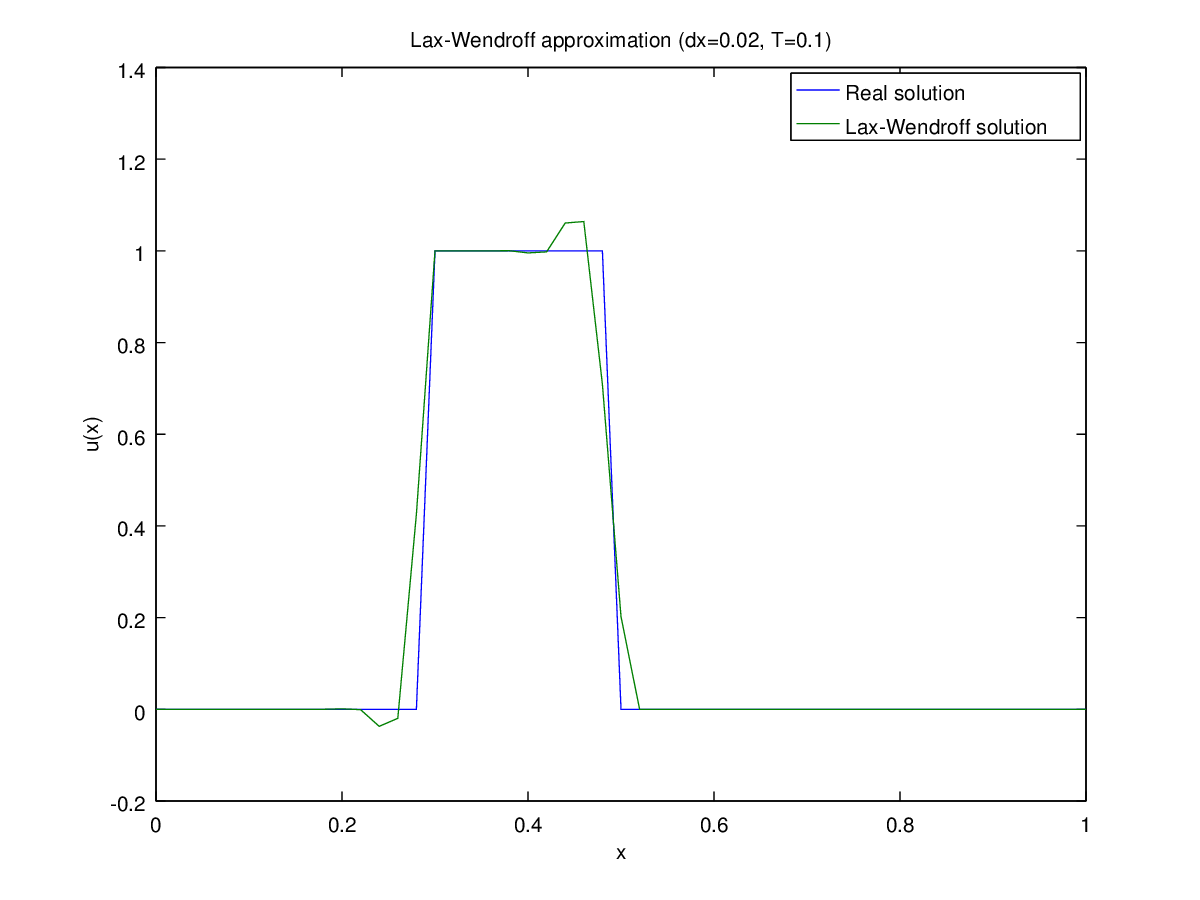
\includegraphics[width=1\linewidth]{../img/lw_1.png}
					\caption{$\Delta x = 0.02$, $T = 0.1$}
					\label{fig:sfig12}
				\end{subfigure}%
				\begin{subfigure}{.7\textwidth}
					\centering
					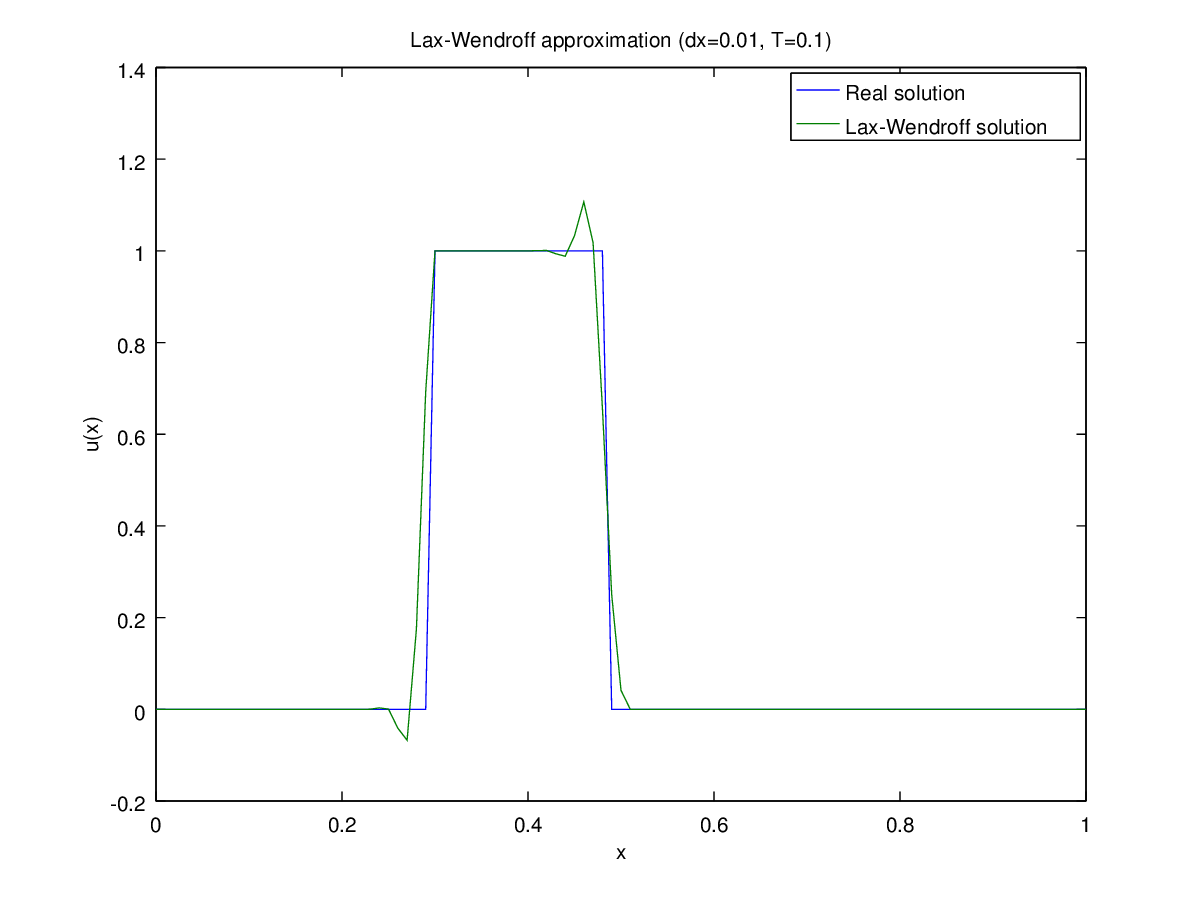
\includegraphics[width=1\linewidth]{../img/lw_4.png}
					\caption{$\Delta x = 0.01$, $T = 0.1$}
					\label{fig:sfig42}
				\end{subfigure}%
			}
			
			\makebox[\textwidth][c]{
				\begin{subfigure}{.7\textwidth}
					\centering
					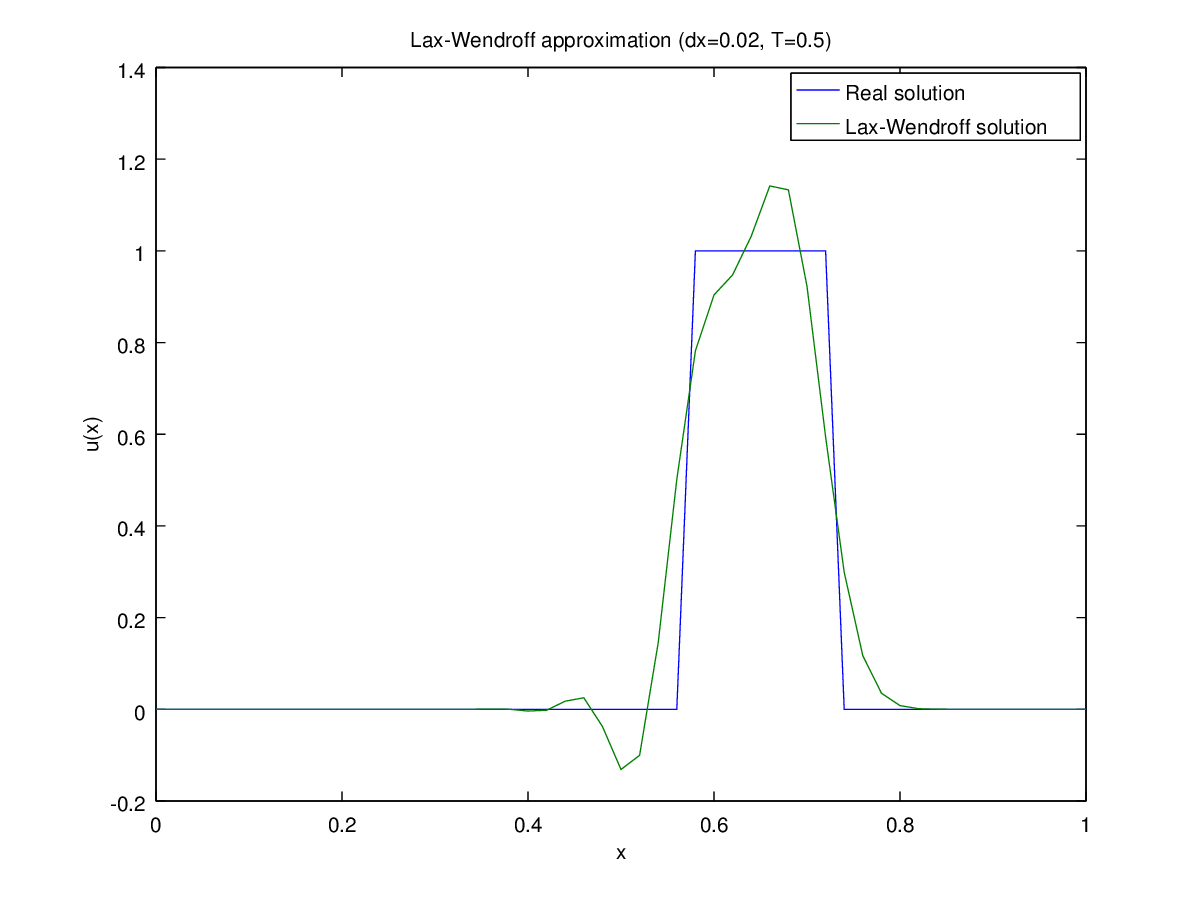
\includegraphics[width=\linewidth]{../img/lw_2.png}
					\caption{$\Delta x = 0.02$, $T = 0.5$}
					\label{fig:sfig22}
				\end{subfigure}%
				\begin{subfigure}{.7\textwidth}
					\centering
					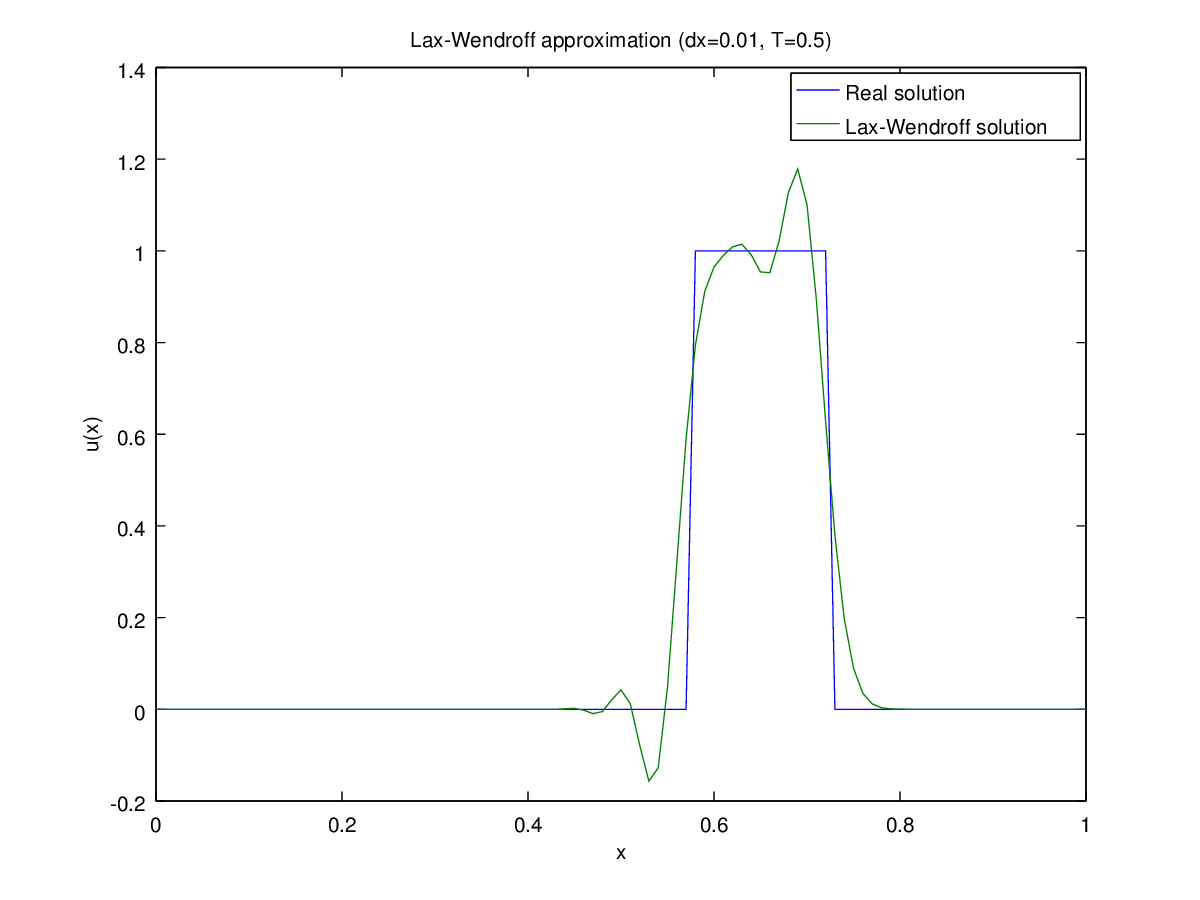
\includegraphics[width=1\linewidth]{../img/lw_5.png}
					\caption{$\Delta x = 0.01$, $T = 0.5$}
					\label{fig:sfig52}
				\end{subfigure}%
			}
			
			\makebox[\textwidth][c]{
				\begin{subfigure}{.7\textwidth}
					\centering
					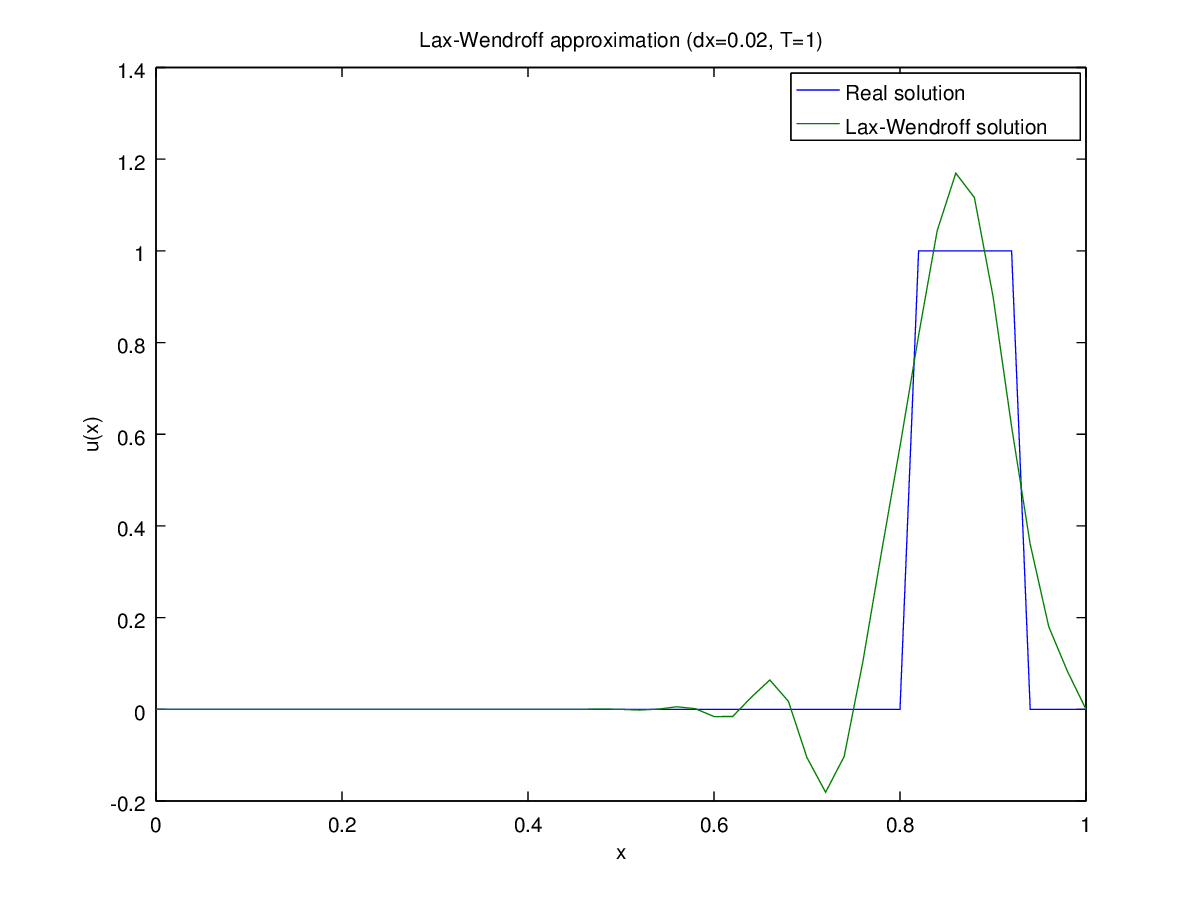
\includegraphics[width=1\linewidth]{../img/lw_3.png}
					\caption{$\Delta x = 0.02$, $T = 1$}
					\label{fig:sfig32}
				\end{subfigure}%
				\begin{subfigure}{.7\textwidth}
					\centering
					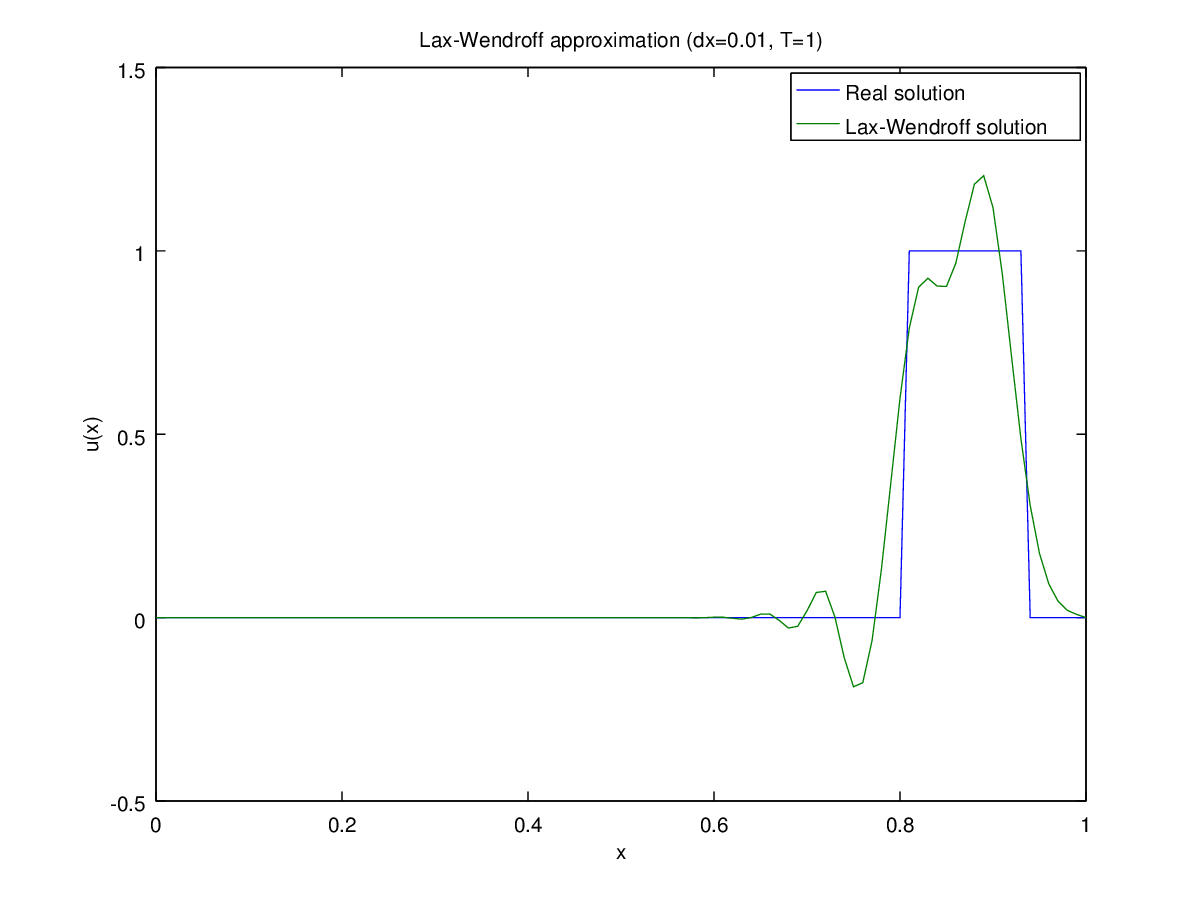
\includegraphics[width=1\linewidth]{../img/lw_6.png}
					\caption{$\Delta x = 0.01$, $T = 1$}
					\label{fig:sfig62}
				\end{subfigure}%
			}
			\caption{Advección lineal utilizando el método Lax-Wendroff.}
			\label{fig:sfig_lw}
		\end{figure}
	\end{center}
	Sabemos que el modo teórico es $e^{-ikat}$ y que el factor de amplificación tiene la expresión
	$$\lambda(k) = \left(1-2\nu^2sin^2\left(\frac{k}{2}\Delta x\right)\right)-i\nu sin(k\Delta x)$$
	Estudiamos el cuadrado del módulo del factor de amplificación:
	$$|\lambda|^2 = 1-4\nu^2(1-\nu^2)sin^4\left(\frac{k}{2}\Delta x\right)$$
	Vemos que para frecuencias bajas, el error en módulo es $\mathcal{O}((k\Delta x)^4)$. En cuanto al error en fase:
	$$\arctan(\lambda(k)) = \arctan\left(\frac{\nu \sin (k\Delta x)}{1-2\nu^2sin^2(\frac{1}{2}k\Delta x)}\right)$$
	Utilizando el lema y desarrollando el polinomio de Taylor obtenemos:
	$$\arctan(\lambda(k)) = -\nu k\Delta x\left[1-\frac{1}{6}(1-\nu^2)(k\Delta x)^2\right]$$
	Luego el error relativo es $\mathcal{O}((k\Delta x)^2)$.
	Se puede observar que este método tiene el mismo orden de error en fase que el esquema upwind pero presenta menos error en módulo. 
	
	En contrapartida, al aumentar la precisión en el módulo el método se comporta mal por no cumplir el principio del máximo.
	Aunque para un mallado más fino hay más precisión en cuanto al módulo de la solución numérica, se puede observar que el hecho de que no se cumpla el principio del máximo resulta en que el método no se comporte bien, presentando oscilaciones. En cuanto al error en la fase, se puede observar que el pulso numérico tiene la velocidad correcta, aunque se observan oscilaciones en los extremos del mismo.
\end{document}